\subsubsection{Donea \& Huerta 2D box geometry benchmark}
\label{sec:benchmark-donea-huerta}

\textit{This section was contributed by Cedric Thieulot.}

This benchmark is taken from Donea and Huerta's book \cite{DH03book}.
The domain is a unit square and the viscosity and density are set to 1.
The components of the gravity vector $\mathbf g$ are prescribed as
\begin{eqnarray}
g_x &=& (12 - 24y) x^4 + (-24 + 48y) x^3 + (-48y + 72y^2 - 48 y^3 + 12) x^2 \nonumber\\
    && + (-2 + 24y -72y^2+48y^3)x + 1-4y + 12y^2-8y^3 \nonumber\\
g_y &=& (8 - 48y + 48 y^2) x^3 + (-12 + 72y - 72y^2) x^2  \nonumber\\
    && + (4 - 24y + 48y^2 - 48y^3 + 24y^4) x - 12y^2 + 24y^3 - 12y^4.
\end{eqnarray}
The exact solution can then be chosen as follows, if one prescribes Dirichlet boundary
values for the velocity using the same formula:
\begin{eqnarray}
u(x,y) &=& x^2(1- x)^2 (2y - 6y^2 + 4y^3)  \nonumber\\
v(x,y) &=& -y^2 (1 - y)^2 (2x - 6x^2 + 4x^3) \nonumber\\
p(x,y) &=& x(1 -x) -1/6.
\end{eqnarray}
Note that the pressure satisfies $\int_{\Omega} p \; \text{d}x = 0$.
The gravity, pressure and velocity fields are shown in Fig.~\ref{fig:doneahuerta-benchmark}.

The convergence of the numerical error of this benchmark has been analyzed by
changing the mesh refinement level in the input file, and
results show that the velocity shows cubic error
convergence, while the pressure shows quadratic convergence in the
$L_2$ norm, as expected when using the $Q_2\times Q_1$ element.

\begin{figure}[t!]
  \centering
  \subfigure[]{
    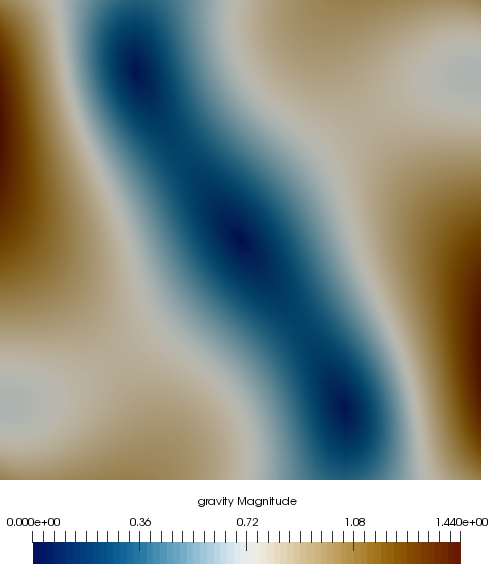
\includegraphics[width=0.31\textwidth]{cookbooks/benchmarks/doneahuerta/doc/grav.png}}%
  ~
  \subfigure[]{
    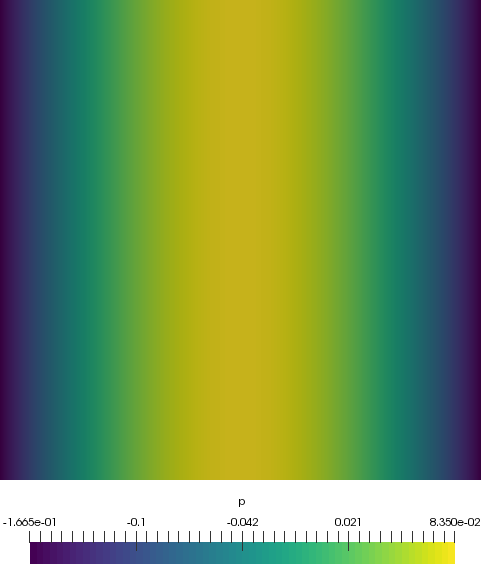
\includegraphics[width=0.31\textwidth]{cookbooks/benchmarks/doneahuerta/doc/press.png}}%
  ~
  \subfigure[]{
    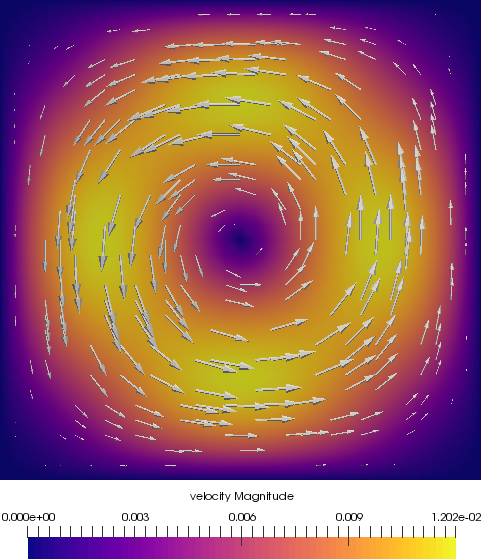
\includegraphics[width=0.31\textwidth]{cookbooks/benchmarks/doneahuerta/doc/vel.png}}
  \caption{\it Donea \& Huerta benchmark: Results for the 2D polynomial Stokes benchmark,
obtained with a resolution of $32\times 32$ elements. (a) Gravity field, (b) pressure field,
(c) velocity field. }\label{fig:doneahuerta-benchmark}
\end{figure}
